\newcommand{\bluearrowDesc}{The blue half-arrow ($\rightharpoondown$) is part of the \acrfull{TLSP}.}

All communication between the Tree Language Server (TLS) and the \gls{VSCode} extension happens over a protocol.
This protocol is part of the artifact design from this thesis, and is called the \acrlong{TLSP}.\\

Because the original \acrshort{EMF} editors are being moved from \gls{Eclipse} to \gls{VSCode}, the protocol draws inspiration from \acrlong{LSP}.
If \gls{Eclipse} already used a \acrshort{LSP}-like language server, the migration would be much easier.
And since it moved once to \gls{VSCode}, it may move again later, for example to IntelliJ (or some other \acrshort{IDE}).\\

The TLSP protocol builds on top the the \textit{Base Protocol} described in \cref{sec:base-protocol}.
That means it sends a header section followed by a content section.
The content has \gls{JSON-RPC} data, being requests, responses, errors, and notifications.
As a reminder: a request must be responded to with a response or error, while a notification does not get an answer.
This means it is a bidirectional communication, where both the extension and the server can initiate a request or notification.
The \acrshort{TLSP} describes what data structures, method names, parameter values and return values should be present in the \gls{JSON-RPC} content.
Because the protocol uses \gls{JSON-RPC} to call the remote procedures, all the data must be serializable to \gls{JSON}.\\

The following subsections present the orders of procedure calls in the \acrshort{TLSP}.
The protocol allows for a stateful server, so for example the workspace must be set before a model is loaded.
The diagrams use UML sequence diagrams.
These have components listed inside boxes at the top, and the timelines as lines coming out below the boxes.
The diagrams are read top to bottom.
A timeline with a box on it represents a process lifetime inside that component.

\subsection{Activation}

Extension activation and document opening is shown in \cref{fig:protocol-startstop}.
When the extension is activated by \gls{VSCode}, the server should be started.
When the server is ready to listen for \acrshort{TLSP} messages, this is indicated by writing a message to an output channel not used for \acrshortpl{TLSP}\footnote{The server uses \textit{standard error} to log and communicate anything that is not \acrshort{TLSP}.}.\\

The extension requests \textit{initialize} with any options the server would need.
The server responds when it is done, allowing the extension to know when it can send the next command.
The workspace path is set to the folder with a student's code.\\

When a \texttt{CustomTreeEditorProvider} in the extension has been asked to open a \texttt{.ecore} document, the server is requested to get the model for this document.
The server responds, and the tree document model is set on the frontend.\\

If the extension is asked to stop, it will first send a \textit{shutdown} request to the server, allowing it to respond when ready to stop.
Then an \textit{exit} notification is sent, which stops the server and breaks the communication.
This shutdown followed by exit procedure is directly inspired by \acrshort{LSP}.


\begin{figure}[htbp]  % order of priority: h here, t top, b bottom, p page
  \centering
  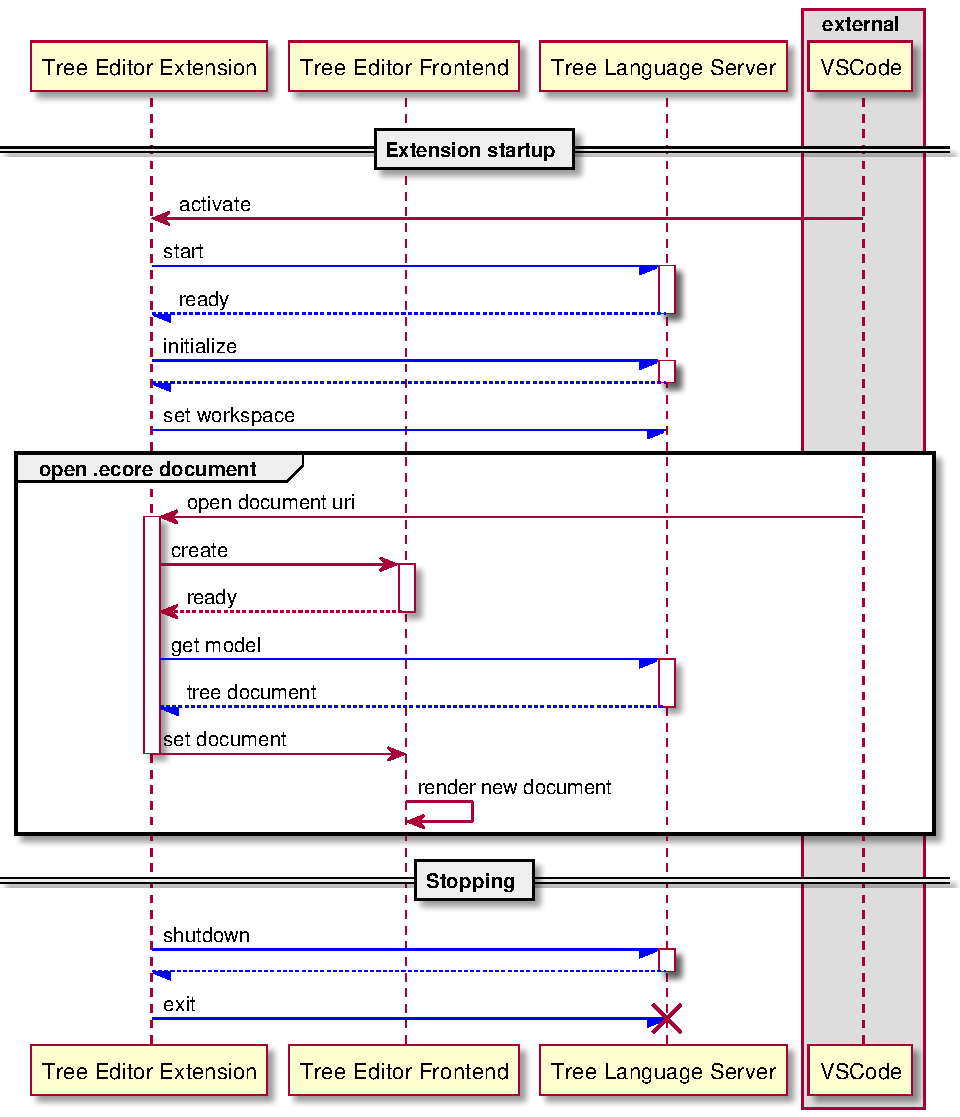
\includegraphics[width=\textwidth]{figures/plantuml/Protocol_startstop_sequence.pdf}
  \caption[Protocol Sequence Diagram of Start/Stop and Document Opening]{Sequence diagram for the protocol when starting and stopping the server. \bluearrowDesc}\label{fig:protocol-startstop}
\end{figure}

\FloatBarrier

\subsection{User Actions}

When a user triggers an action from the frontend, such as validation or code generation, an \texttt{ActionEvent} is sent to the server.
If this event changes the model, a notification will be sent by the server to update the document state.
This is shown in \cref{fig:protocol-action}.

\begin{figure}[htbp]  % order of priority: h here, t top, b bottom, p page
  \centering
  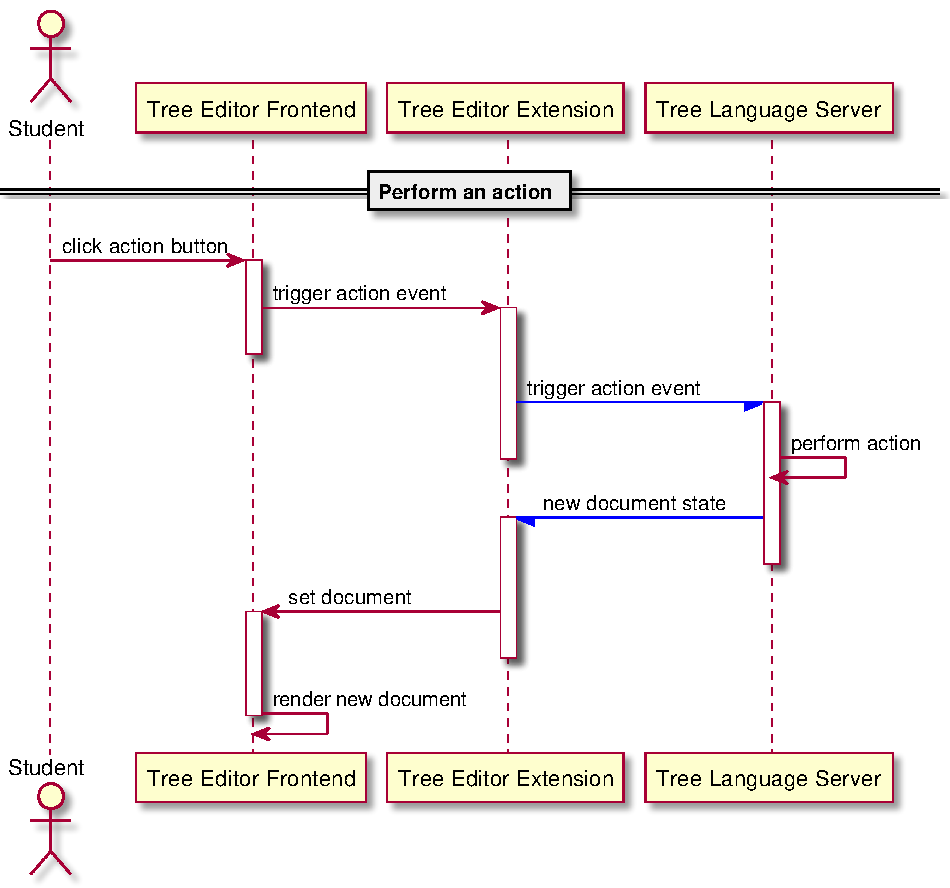
\includegraphics[width=\textwidth]{figures/plantuml/Protocol_action_sequence.pdf}
  \caption[Protocol Sequence Diagram of Action Triggering]{Sequence diagram for the protocol when triggering an action. \bluearrowDesc}\label{fig:protocol-action}
\end{figure}

\FloatBarrier

\subsection{Property Editing}

When a student wants to modify a model element, they first have to select the corresponding tree node.
When the selection changes, the frontend asks the extension for the properties of that node.
This request is then sent to the server, where it returns both the node properties and the schema for JSON-Forms to present it.
This is shown in \cref{fig:protocol-form}.\\

Then when the properties of the node are changed, an event is sent to the server indicating the id of the node and the new property values.
This is shown in the lower half of \cref{fig:protocol-form}.

\begin{figure}[htbp]  % order of priority: h here, t top, b bottom, p page
  \centering
  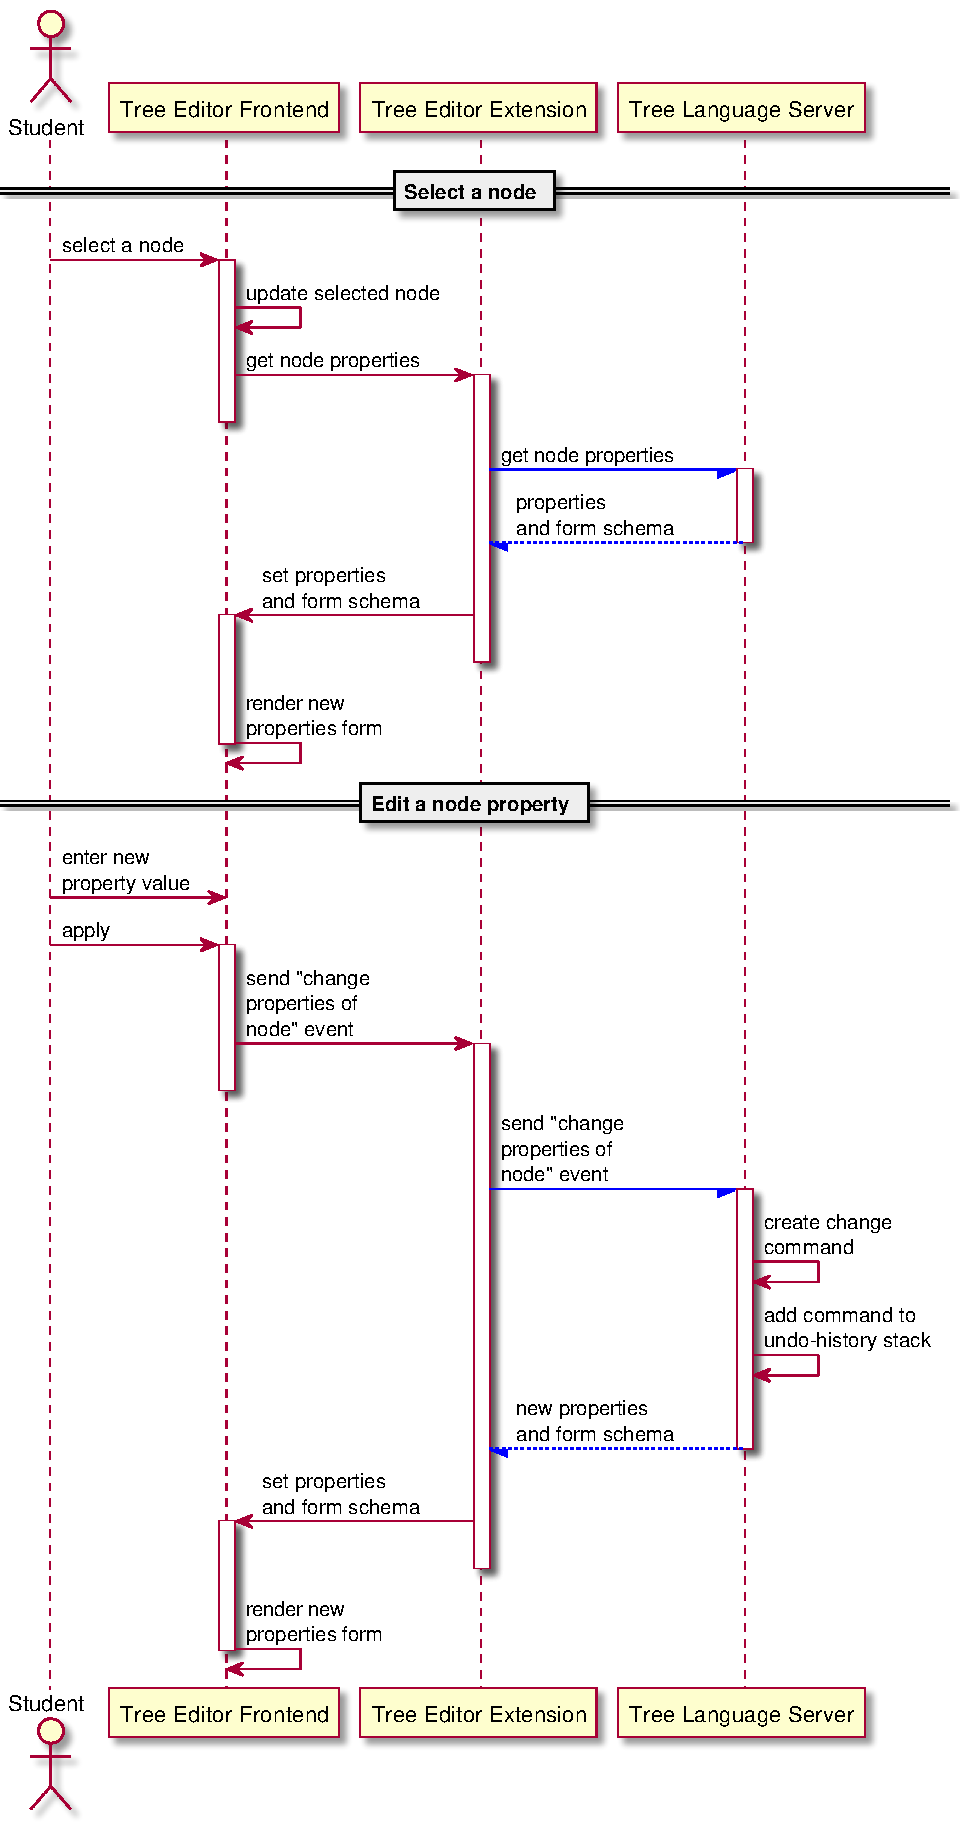
\includegraphics[width=\textwidth,height=\textheight,keepaspectratio]{figures/plantuml/Protocol_form_sequence.pdf}
  \caption[Protocol Sequence Diagram of Property Form]{Sequence diagram for the protocol when editing a node property. \bluearrowDesc}\label{fig:protocol-form}
\end{figure}

\FloatBarrier

\subsection{Tree Editing}

Editing the tree hierarchy by adding children is done by first selecting the child node's type.
This can be presented using the \texttt{HierarchySchema}, which is already sent on the \texttt{TreeDocument} when the model was loaded.
When a student selects the node to add a child on, and the type of child node, this is sent via the extension towards the server.
The server should create a \texttt{Command} from the \texttt{.edit} framework, in order to have a undo/redo history.
The new document state is returned afterwards.
This is shown in \cref{fig:protocol-changetree}.

\begin{figure}[htbp]  % order of priority: h here, t top, b bottom, p page
  \centering
  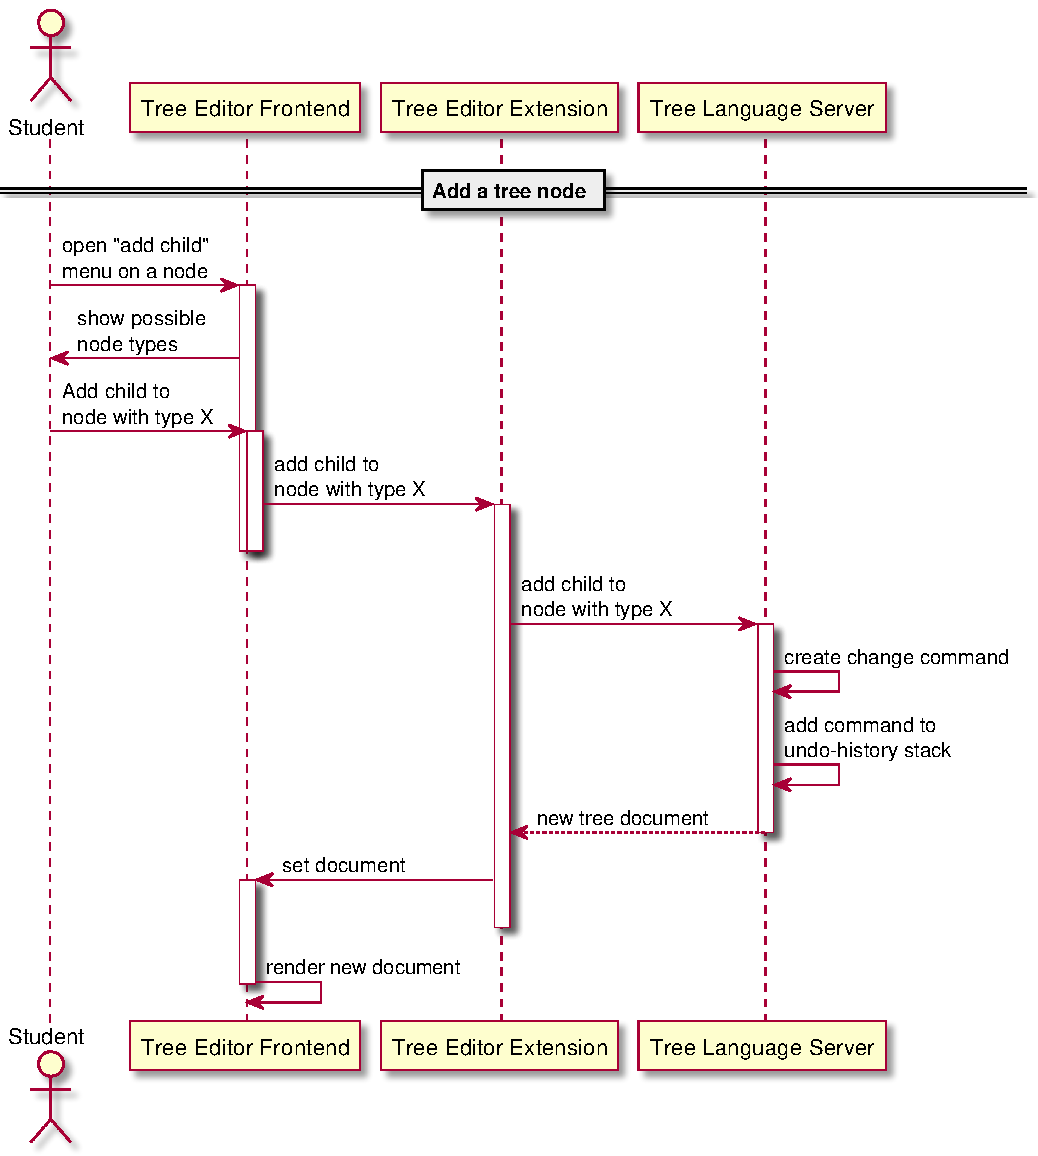
\includegraphics[width=\textwidth]{figures/plantuml/Protocol_changetree_sequence.pdf}
  \caption[Protocol Sequence Diagram of Tree Changes]{Sequence diagram for the protocol when adding a child node. \bluearrowDesc}\label{fig:protocol-changetree}
\end{figure}


\FloatBarrier
